
\section{Experiments }
%\subsection{Implementation}
\subsubsection{New environment}

{\color{red}Since   source code and execution files  
	of    \eign, \cf,  \sle\  can not be found in public area at now, we only compare \froot\ with \AND, \MM's \inte\  and  \MAPLE's \REALROOT\  on   a 64-bit Intel(R) Core(TM) i7 CPU-4710Q @ 2.50GHz with 8GB RAM memory and Windows 7. In this environment \froot\ compiled by visual studio 2013}.

\subsubsection{Old environment}
The main algorithm for isolating real roots based on our improvements has been implemented as a \texttt{C} program, \froot \footnote{The program can be downloaded through \url{https://github.com/djuanbei/logcf}}. Compilation was done using {\tt gcc} version 4.6.3 with optimization flags -O2.
We use {\tt Singular} \cite{singular} to read polynomials from files or standard input and to eliminate multi-factors of polynomials. We use the GMP\footnote{ \url{http://gmplib.org/}}
(version 5.05), arbitrary-length integers libraries, to deal with big integer computation.
Some of test did before 2014   on a 64-bit Intel(R) Core(TM) i5 CPU 650 @ 3.20GHz with 4GB RAM memory and Ubuntu 12.04 GNU/Linux.



\subsection{Benchmarks }
 \subsubsection{$W_n$}
 {\it Wilkinson} polynomials: $W_n=\Pi_{i=1}^n(x-i)$. The integers $1,2,\ldots,n $ are  all the real roots of $W_n$.
  \subsubsection{$mW_n$}
  %{\it Wilkinson}  polynomials have a fine property  of containing only rational roots, which most of the polynomials do not have . So we modify
  Modified {\it Wilkinson} polynomials: $mW_n=W_n-1$.

  If $n>10$, $mW_n$ has $n$ simple real roots but most of them are irrational.
 \subsubsection{$IW_n$}
 The distance between  $W_n$'s two  nearest real roots  is  $1$ and the distance between $mW_n$'s two nearest real roots  is nearly $1$. %Their real roots distribution   tends to be  uniform.  So
 We construct new polynomials $IW_n=\Pi_{i=1}^n(ix-1)$, which have a completely different distance between any two nearest real roots.
 \subsubsection{$ mIW_n$ }
 We modify $IW_n$  into $mIW_n=IW_n-1$ for the same purpose  as we construct $mW_n$. Most real roots of $mIM_n$  become irrational.
 \subsubsection{$T_n$} {\it ChebyshevT} polynomials: $T_0=1,T_1=x,T_{n+1}=2xT_n-T_{n-1}$. $T_n$ has $n$ simple real roots.
 \subsubsection{$U_n$} {\it ChebyshevU} polynomials: $U_0=1,U_1=2x,U_{n+1}=2xU_n-U_{n-1}$. $U_n$ has $n$ simple real roots.
 \subsubsection{$L_n$}
 {\it Laguerre}  polynomials: $L_0=1$,$L_1=1-x$,$L_{n+1}(x)=\frac{  (2n+1-x )L_n(x)-  nL_{n-1 }(x)}{(n+1) }$. %We can
 %modify  it to  integer polynomial through multiplying   by  $n!L_n$.
Obviously, $n!L_n$ is a polynomial with integer coefficients.
 \subsubsection{$M_n$} {\it Mignotte} polynomials: $x^n-2(5x-1)^2$. If $n$ is odd, $M_n$ has three simple real roots. If $n$ is even, it has four simple real roots.

\subsubsection{$MR_n$}{\it Mignotte} rational center polynomials: $ x^n-((2^7-1)x-1)^2$.
	 
 \subsubsection{$H_n$}{\it Hermite } polynomials:  $H_0=1,H_1=2x,H_n=2xH_{n-1}-2(n-1)H_{n-2}$. $H_n$ has $n$ simple real roots.
 
 \subsubsection{$MI_n$} {\it Mignotte} irrational center polynomials: $x^{129}-((2^{\frac{1}{4}n}-1)x^2-1)^2$.
 
 
 \subsubsection{$R(n,b,r) $} Randomly generated polynomials: $R(n,b,r)$=$a_nx^n+\cdots+a_1x+a_0$ with $|a_i|\le b, Pr[a_i\ge 0]=\frac{1}{2}$ and  $Pr[a_i\neq 0] =1-r,$ where $Pr$ means probability.
 \subsection{Results}
 The root isolation timings in Tables \ref{tab:open} are in seconds.  Most of the benchmarks we chose have large degrees and the timings show that our tool is very efficient.
% some  applications of isolation real roots produce very large degree polynomials, such as quantifier elimination.
 {\color{red} As a  built-in  \MAPLE\ function, \REALROOT\ is    compared with  our tool \froot. 
 	The   \MAPLE\  we use has a version number 2017.}  For  almost all
 benchmarks, our  software \froot\  can be  four  times faster than \REALROOT. The comparative data can be found in Figure \ref{fig:r} and Figure \ref{fig:2}. {\color{red} In many cases, \froot\ is much faster than \REALROOT, the mean speedup is more than $4$ and the largest speedup is more than $15$.}
 
 
 As a  built-in \MM\ symbol, \inte\ is    compared with  our tool \froot. The  \MM\  we use has a version number 11.1. {\color{red} In some of cases \inte\ is faster than \froot, but we find a bug of  \MM\  during we test. In Table  \ref{tab:and} when $n=1024,1448,2096$  \inte's ouput that there a double. We analysis the reason for this \inte's failure is that \inte\ uses {\tt PossibleZeroQ} to check whether an expression is zero or not but  {\tt PossibleZeroQ} can not guarantee its output.}
 
 
 We also consider open software,  such as \cf\  \cite{hemmer09}, \AND\cite{Tsigaridas2016}, \SLV\cite{kobel2016computing}  which
 seem to be the fastest  open softwares  available for exact real root isolation. Many experiments  about  state of the art open software for isolating
 real roots have been done in \cite{hemmer09,Tsigaridas2016,kobel2016computing},  which  indicate that     \cf, \AND, \SLV\ 
 are  the fastest in many cases.
 In our experiments, \froot\ is much faster than \cf. %We only consider a few of benchmarks with only simple roots as they can indicate  difference between two softwares.
 The comparative result can be found in
 Table \ref{tab:open}. {\color{red}\froot\ is speedup between $2$ and $200$ compare with \cf.  In Figure \ref{fig:r} and Figure \ref{fig:2}, \froot\ is about $4$ times faster than \AND\ and the maximum speedup is more than $15$. Compared with \SLV, \froot\  is mean $4000$ times faster on $MR_n$ polynomials,  $10$ times faster on  \SLV\ on $W_n,T_n,U_n,H_n$ polynomials and  $4$ times faster  on $M_n$ polynomials. Under $MI_n$ polynomials \froot\ is about $4$ times slower than \SLV. }
 
 
  We also compare \froot\  with numerical methods  \eign\ \cite{eigsolev} and \sle\ \cite{hemmer09}. As \eign\ computes all the complex roots, we choose $W_n$, $mW_n$ and $IW_n$ as benchmarks with degrees ranging from 10 to 90, which have only real roots. \sle\ computes only real roots but it has weak stability. Its output on $W_{30}$ only has eight real roots, which is obviously wrong. \sle's running time\footnote{When  running time is very short we run every case for more than ten times and compute the mean.} on $W_{10}$ is $0.022$ seconds and
 $0.024$ seconds on $W_{20}$. In these two cases our software is about $7$ times faster than \sle. We compare \froot\ with  \eign\ and the results are  shown in Figure \ref{fig:1}.
 At the beginning when degree is $10$, the time costs of \froot\ and \eign\ are
 almost equal. As degree becoming larger, the growth rate of our tool's consuming-time is much less than that of  \eign.  When degree reaches $90$, \froot\ is about $20$ times faster than \eign.


%
% \begin{table}[H]
%  \centering
%  \captionof{table}{Compare with \MM(1) on old environment }
%  \label{tab:mm1}
%  %\tbl{Compare with \MM(1)\label{tab:mm1}}{
%  \begin{tabular}{|| c| c| c|| c|c| c||}
%\hline
%\scriptsize{Benchmark}  & \scriptsize{\inte}  &\scriptsize{ \froot} &\scriptsize{Benchmark}  & \scriptsize{\inte}  &\scriptsize{ \froot}\\
%\hline
%$W_ {100}$ & 0.024 & 0.01 & $ IW_{100}$ & 0.048 & 0.01\\
%\hline
%$W_{200}$ & 0.096 & 0.015 & $IW_{200}$ & 0.148 & 0.015\\
%\hline
%$W_{300}$ & 0.19 & 0.03 &$IW_{300}$ & 0.33 & 0.03\\
%\hline
%$W_{400}$ & 0.36 & 0.06 & $IW_{400}$ & 0.72 & 0.08\\
%\hline
%$W_{ 500}$ & 0.624 & 0.11& $IW_{500}$ & 1.2 & 0.13\\
%
%\hline
%$W_{ 1000}$ & 3.33 & 0.87& $IW_{1000}$ & 5.53 & 0.86\\
%
%\hline
%$W_{2000}$ & 21.58 & 6.88& $IW_{ 2000}$ & 26.08 & 8.28\\
%\hline
%$mW_{100}$ & 0.084 & 0.025& $mIW_{100}$ & 0.032 & 0.01\\
%
%\hline
%$mW_{ 200}$ & 0.55 & 0.16& $mIW_{200}$ & 0.172 & 0.04\\
%
%\hline
%$mW_{300}$ & 1.92 & 0.63& $mIW_{300}$ & 0.548 & 0.16\\
%
%\hline
%$mW_{400}$ & 4.92 & 1.77 & $mIW_{400}$ & 1.30 & 0.44\\
%
%\hline
%$mW_{500}$ & 10.6 & 4.34 & $mIW_{500}$ & 2.73 & 1.01\\
%
%\hline
%$mW_{1000}$ & 140.9 & 65.62 &$ mIW_{1000}$ & 32.9 & 15.56\\
%\hline
%  \end{tabular}%}
%\end{table}
%
%
%\begin{table}[H]
%  \centering
%  \captionof{table}{compare with \MM(2) on old environment } \label{tab:mm2}
%  %\tbl{ compare with \MM(2) \label{tab:mm2}}{
%  \begin{tabular}{||c| c| c|| c| c| c|| }
%\hline
%
%\ \scriptsize{Benchmark}\   & \scriptsize{\inte}  &\scriptsize{ \froot} &\ \scriptsize{Benchmark}\   & \scriptsize{\inte}  &\scriptsize{ \froot}\\
%%Benchmark  &\inte  & \froot & Benchmark  &\inte & \froot\\
%
%\hline
%
%$T_{100}$&  0.056 &  0.01 & $L_{100}$&  0.072 & 0.02  \\
%
%\hline
%$T_{200}$&  0.39 &  0.03& $L_{200}$  & 0.60 &0.16 \\
%
%\hline
%$T_{300}$  & 1.29 & 0.10& $L_{300}$  & 2.2 &0.69 \\
%
%\hline
%$T_{400}$ & 3.39 &  0.22& $L_{400}$ & 5.64 &1.91 \\
%
%\hline
%$T_{500}$ & 7.26 & 0.45& $L_{500}$  & 12.24 &4.59 \\
%
%\hline
%$T_{1000}$ & 90.8 & 4.96& $L_{1000}$  & 150 &72.3 \\
%\hline
%
%$U_{100}$  & 0.048 &  0.01& $M_{2000}$  & 1.22 & 0.19 \\
%
%\hline
%$U_{200}$ & 0.35 &  0.03& $M_{2001}$ & 1.22 & 0.20 \\
%
%\hline
%$U_{300}$ & 1.31 & 0.09& $M_{4000}$ & 8.02 & 1.79 \\
%
%\hline
%$U_{400}$ & 3.35 &  0.21& $M_{4001}$ & 7.98 & 1.99 \\
%
%\hline
%$U_{500}$ & 6.95 & 0.44& $M_{6000}$ & 33.4 & 7.73 \\
%
%\hline
%$U_{1000}$ & 87.5 & 4.81&  $M_{6001}$ & 33.7 & 7.82 \\
%\hline
%  \end{tabular}%}
%\end{table}


%\subsection{ Randomly generated benchmarks}
%\subsubsection*{ Randomly generated benchmarks}

For randomly generated polynomials, we consider different settings of
$(n,b,r)$ as shown in Figure \ref{fig:2}. For each setting $(n,b,r)$, we generate randomly five instances and  compute the mean of five running times. In almost every randomly generated benchmark our \froot\  is  faster than other  solvers. And We can also  find that
degree is the main factor affecting the  running time.

{\color{red} More test result can be found in
	
	 \url{https://github.com/djuanbei/logcf/blob/master/testresult.xls}}

\begin{table}[H]
  \centering
  %\tbl{    compare with \cf  \label{tab:open}}{
  \captionof{table}{ compare with \cf\ on old environment } \label{tab:open}
  \begin{tabular}{|| c| c| c|| c|c| c||}
\hline

\hline
\scriptsize{Benchmark}  &\ \  \ \    \ \ \scriptsize{\cf}\ \  \ \  \ \     & \scriptsize{\froot} &\scriptsize{ Benchmark}  &\ \   \ \ \ \  \ \scriptsize{ \cf} \  \  \ \ \ \    \    & \scriptsize{\froot}\\
\hline
$W_{100}$ & 0.054 & 0.01 &  $IW_{100}$ & 0.056 & 0.01\\
\hline
$W_{200}$ & 0.23 & 0.015 & $IW_{200}$ & 0.20 & 0.015\\
\hline
$mW_{100}$ & 0.054 & 0.025& $mIW_{100}$ & 0.14 & 0.01\\
\hline
$mW_{200}$ & 40.5 & 0.16& $mIW_{200}$ & 2.7 & 0.04\\
\hline
$T_{100}$ & 0.52 &  0.01 & $L_{100}$ & 0.80 & 0.02  \\

\hline
$T_{200}$ & 4.32 &  0.13& $L_{200}$ & 7.50 &0.16 \\

\hline
$U_{100}$ & 0.52 &  0.01& $M_{1000}$ & 43.52 & 0.03 \\

\hline
$U_{200}$ & 4.15 &  0.12& $M_{1200}$ & 88 & 0.05 \\

\hline

\hline
  \end{tabular}%}
\end{table}


\begin{figure}[!ht]
	\begin{centering}
		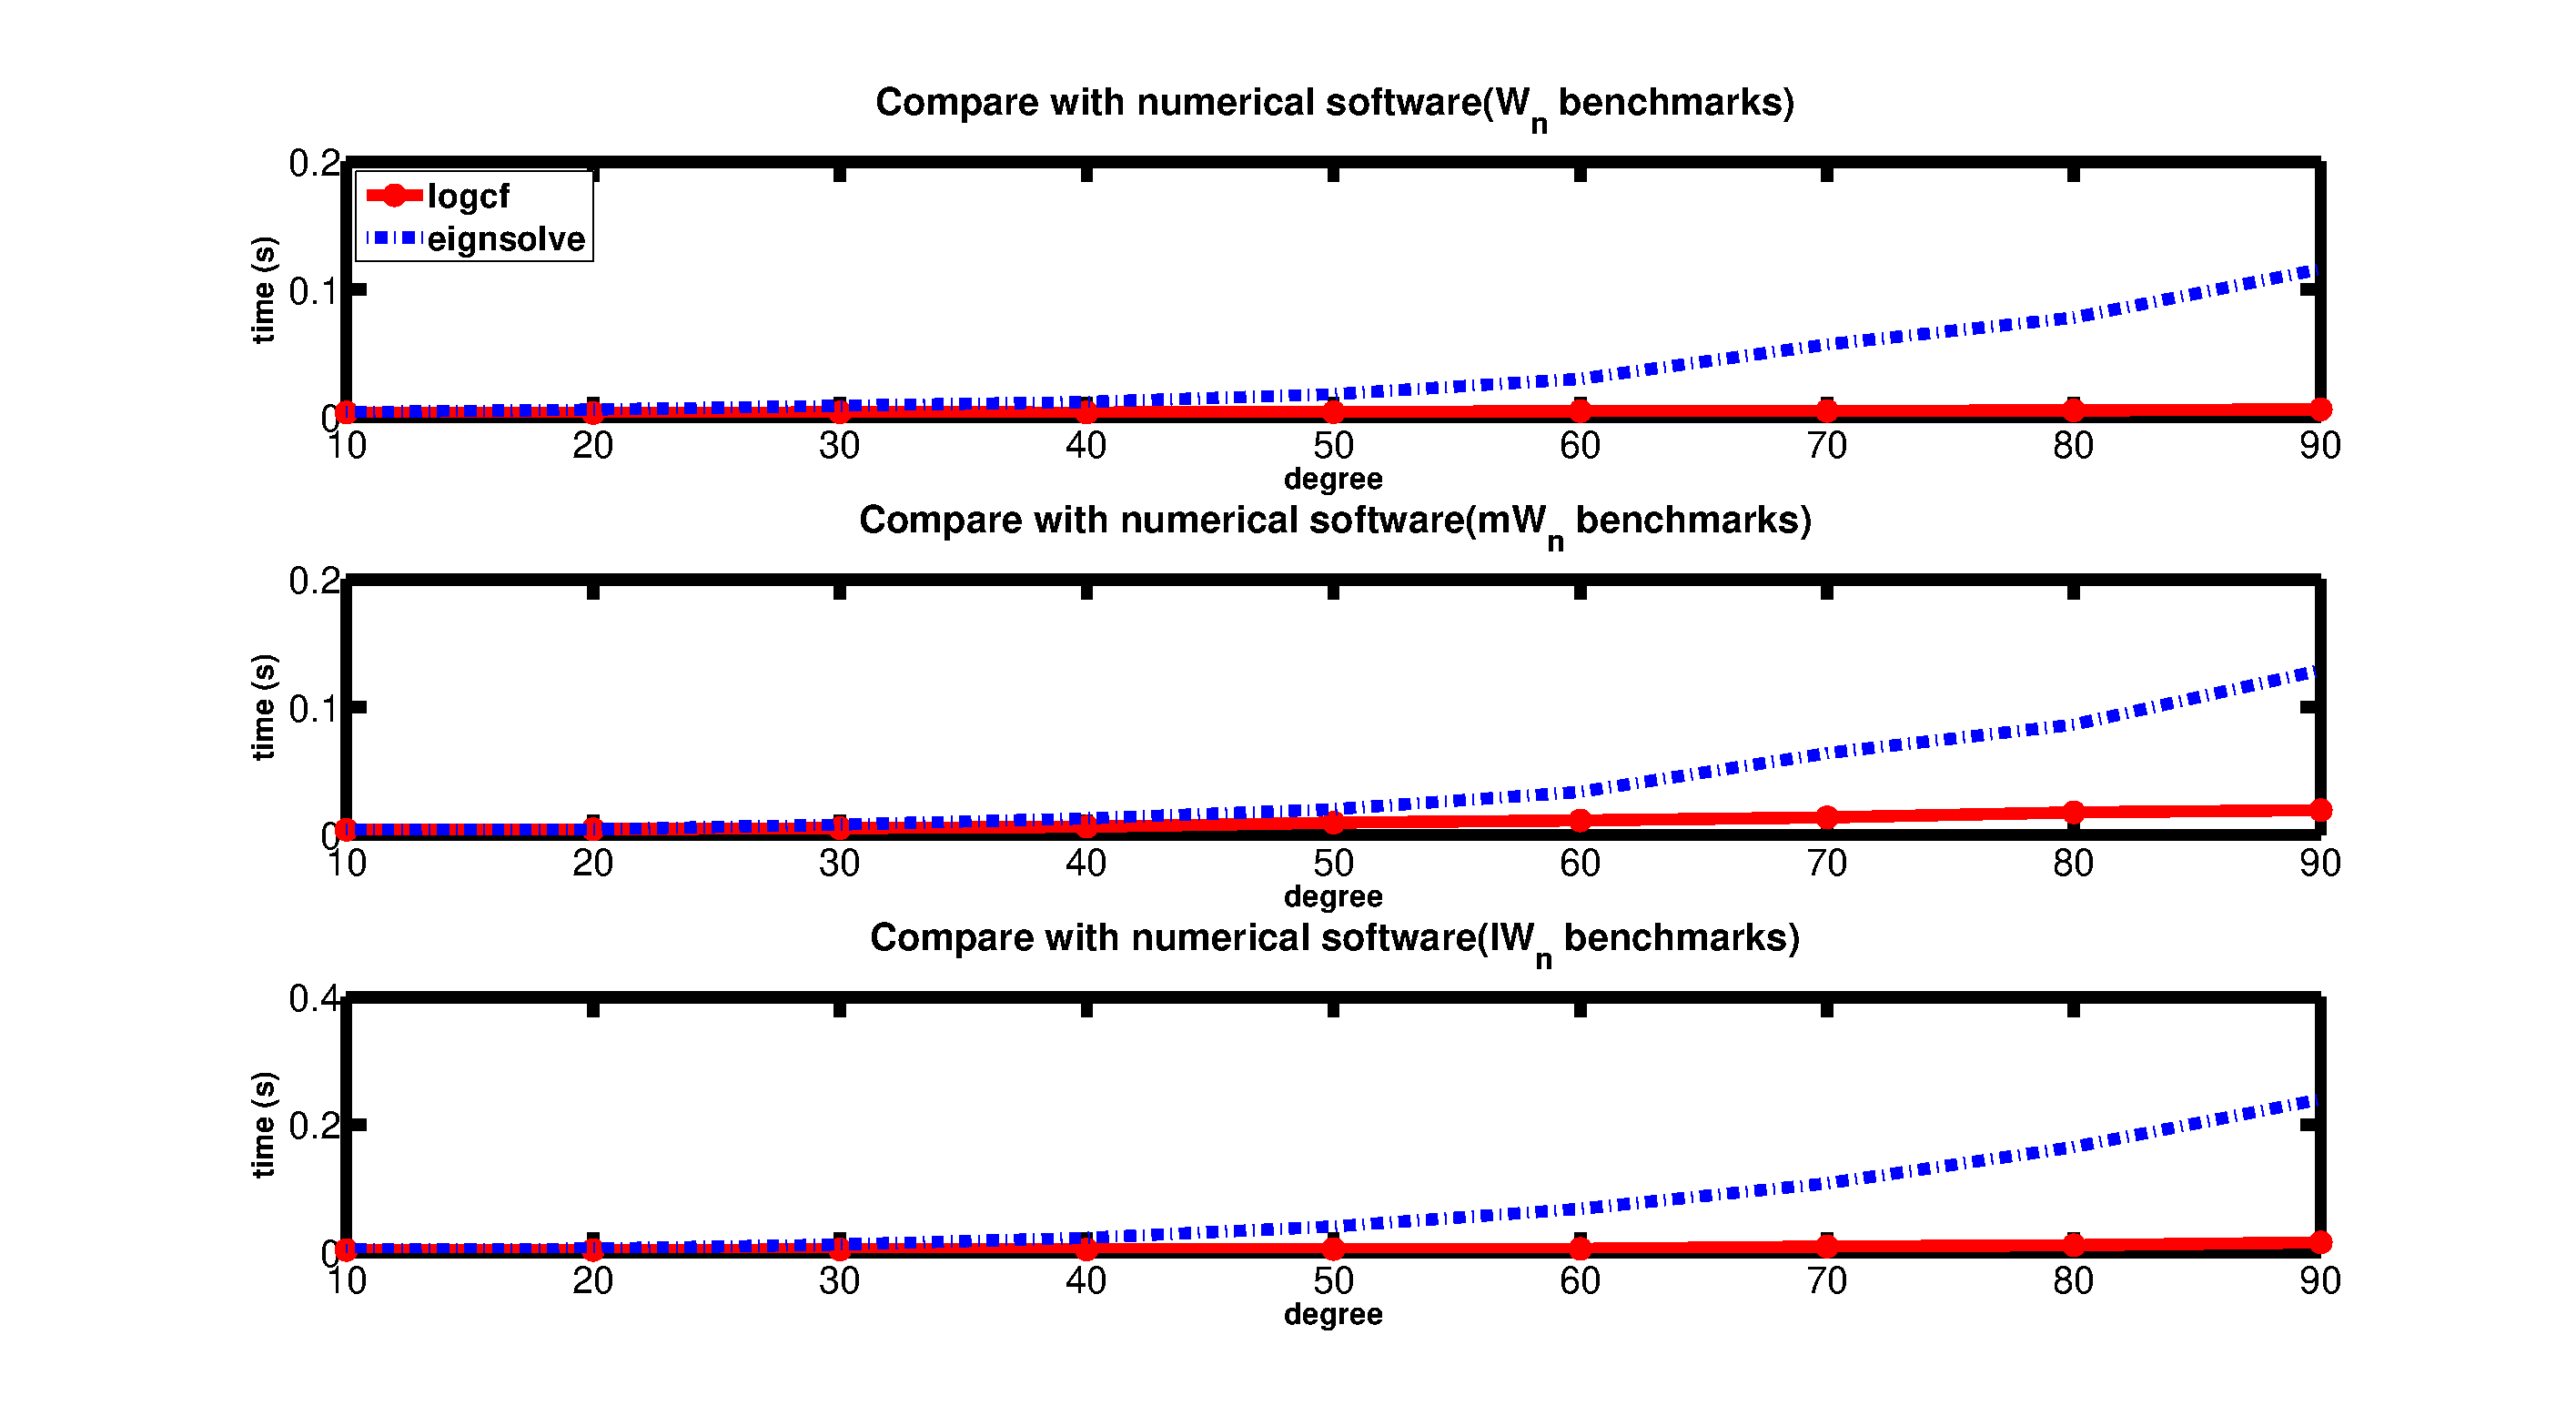
\includegraphics[width=5.4in]{com}
		\caption{ compare with numerical software  \eign\  on old environment\label{fig:1}}
	\end{centering}
\end{figure}




\begin{table}[H]
	\centering
	\captionof{table}{Run time(s) on $MR_n$ polynomails on new environment} 
	\label{tab:and}
	\begin{tabular}{|| c| c| c| c| c ||}
		\hline
		
		\hline
		\scriptsize{Degree}  &\ \  \ \ \ \ \scriptsize{\froot}\ \  \ \  \ \   & \scriptsize{\REALROOT} &\scriptsize{\inte}  &\ \   \ \    \scriptsize{\AND}\ \ \ \   \\
		\hline
		$128$ & 0.016 & 0.734 &  0.015 &  0.02\\
		\hline
		$181$ & 0.018 & 11.154 & 0.031 & 0.038\\
		\hline
		$256$ & 0.034 & 94.849&  0.046  & 0.063\\
		\hline
		$362$ & 0.083 & >600&  0.094 & 0.11\\
		\hline
		$512$ & 0.20 &  >600 & 0.219 & 0.20  \\
		
		\hline
		$724$ & 0.55 &  >600&  0.344 & 0.42 \\
		
		\hline
		$1024$ & 1.46 & >600& {\color{red}error} & 0.79 \\
		
		\hline
		$1448$ & 6.48 &  >600&  {\color{red}error} &  1.69 \\
		\hline
		$2096$ & 24.19 &  >600&  {\color{red}error} & 3.16 \\	
		\hline
		
		\hline
	\end{tabular}%}
\end{table}


\begin{figure}[!ht]
	\begin{centering}
		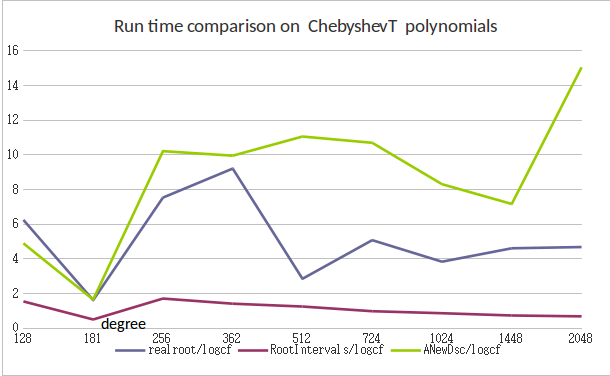
\includegraphics[width=4.4in]{Tn}
		\caption{ compare about solving ChebyshevT polynomials on new environment\label{fig:r}}
	\end{centering}
\end{figure}


%\begin{figure}[!ht]
%	\begin{centering}
%		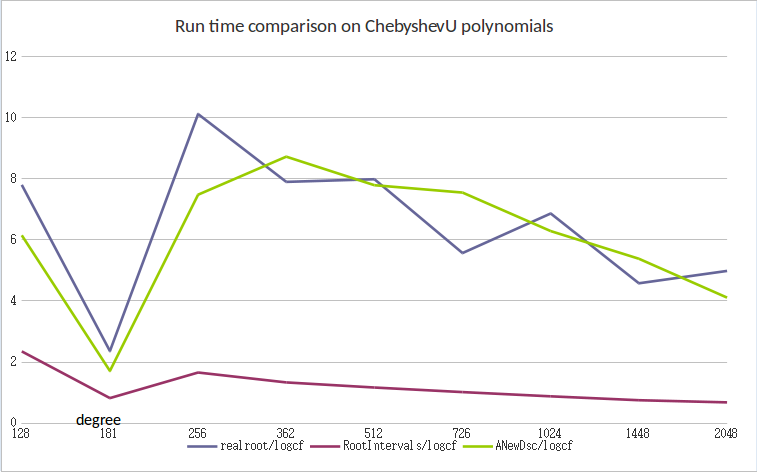
\includegraphics[width=4.4in]{Un}
%		\caption{ compare about solving ChebyshevU polynomials on new environment\label{fig:u}}
%	\end{centering}
%\end{figure}
%
%
%\begin{figure}[!ht]
%	\begin{centering}
%		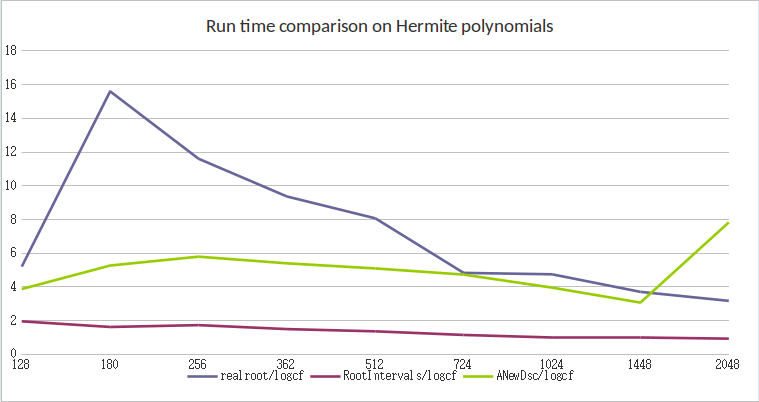
\includegraphics[width=4.4in]{Hn}
%		\caption{ compare about solving Hermite polynomials on new environment\label{fig:h}}
%	\end{centering}
%\end{figure}


%
%\begin{figure}[!ht]
%	\begin{centering}
%		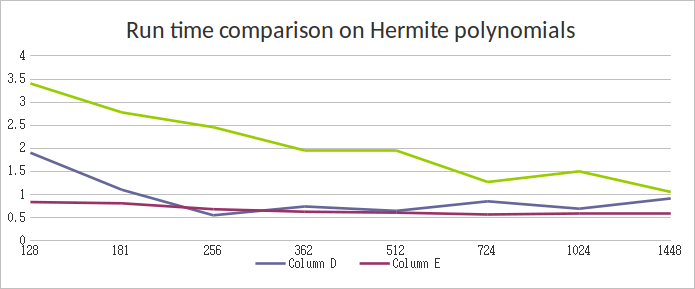
\includegraphics[width=4.4in]{Wpn}
%		\caption{ compare about solving Hermite polynomials on new environment\label{fig:h}}
%	\end{centering}
%\end{figure}





\begin{figure}[!ht]
\begin{centering}
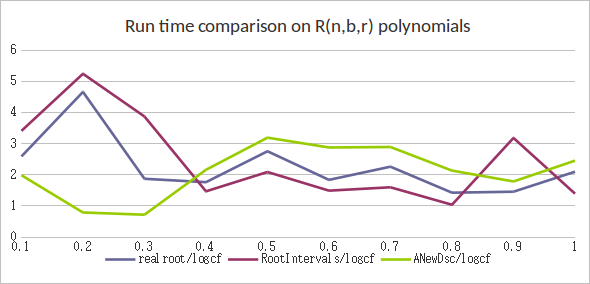
\includegraphics[width=4.4in]{Rn}
\caption{ $R(n,b,r)$ benchmarks  with differ setting on new environment\label{fig:2}}
\end{centering}
\end{figure}

